\section{Applications and Real-world deployment experiences} \label{sec:rbnb-apps-experiences}

In this section, we present some selected experiences in deploying the DataTurbine for observing systems. 

\subsection{Earthquake engineering experiment}
Variations in the configuration of RBNB servers and RBNB clients are simple to implement. It is just a matter of making the desired connections at the start of the experiment. For example, % in an 
for an experiment on the stresses caused by earthquakes, collaborating scientists
%the University of California, Los Angeles (UCLA) 
instrumented a building  damaged in the Northridge earthquake.  

The experiment consisted of 16 channel DAQ card, being used in differential mode to yield 8 channels. These were 4-way multiplexed to read 32 strain gages using a sample-and-hold buffer in the SCXI chassis. There were three separate such systems, for a total of 96 channels of strain gage data. In addition, there were a number of accelerometers connected to Quanterra Q330 dataloggers via Antelope ~\cite{BRTT}. We wrote an adapter to communicate with the Antelope system and retrieve the data for insertion into DataTurbine.

In this collaborative experiment the field site was equipped with a satellite uplink and the goal was to stream data and video to a large number of clients. The satellite link was 1.5Mbps, therefore we need to send exactly one copy across that link. To solve this, we used the 'parent-child' routing feature of the DataTurbine, where the 'parent' resided on a server on-campus and the child was on a Linux server onsite. Data was streamed to the child machine, went across the satellite link via the routing, and the clients all connected to the parent on campus. This avoided saturating the satellite link, see Figure~\ref{fig:ucla-arch}) for a schematic. Remote users could view data via the turbine on campus without affecting the onsite RBNB server.

\subsection{Telepresence}

\begin{figure*}
% \begin{center}
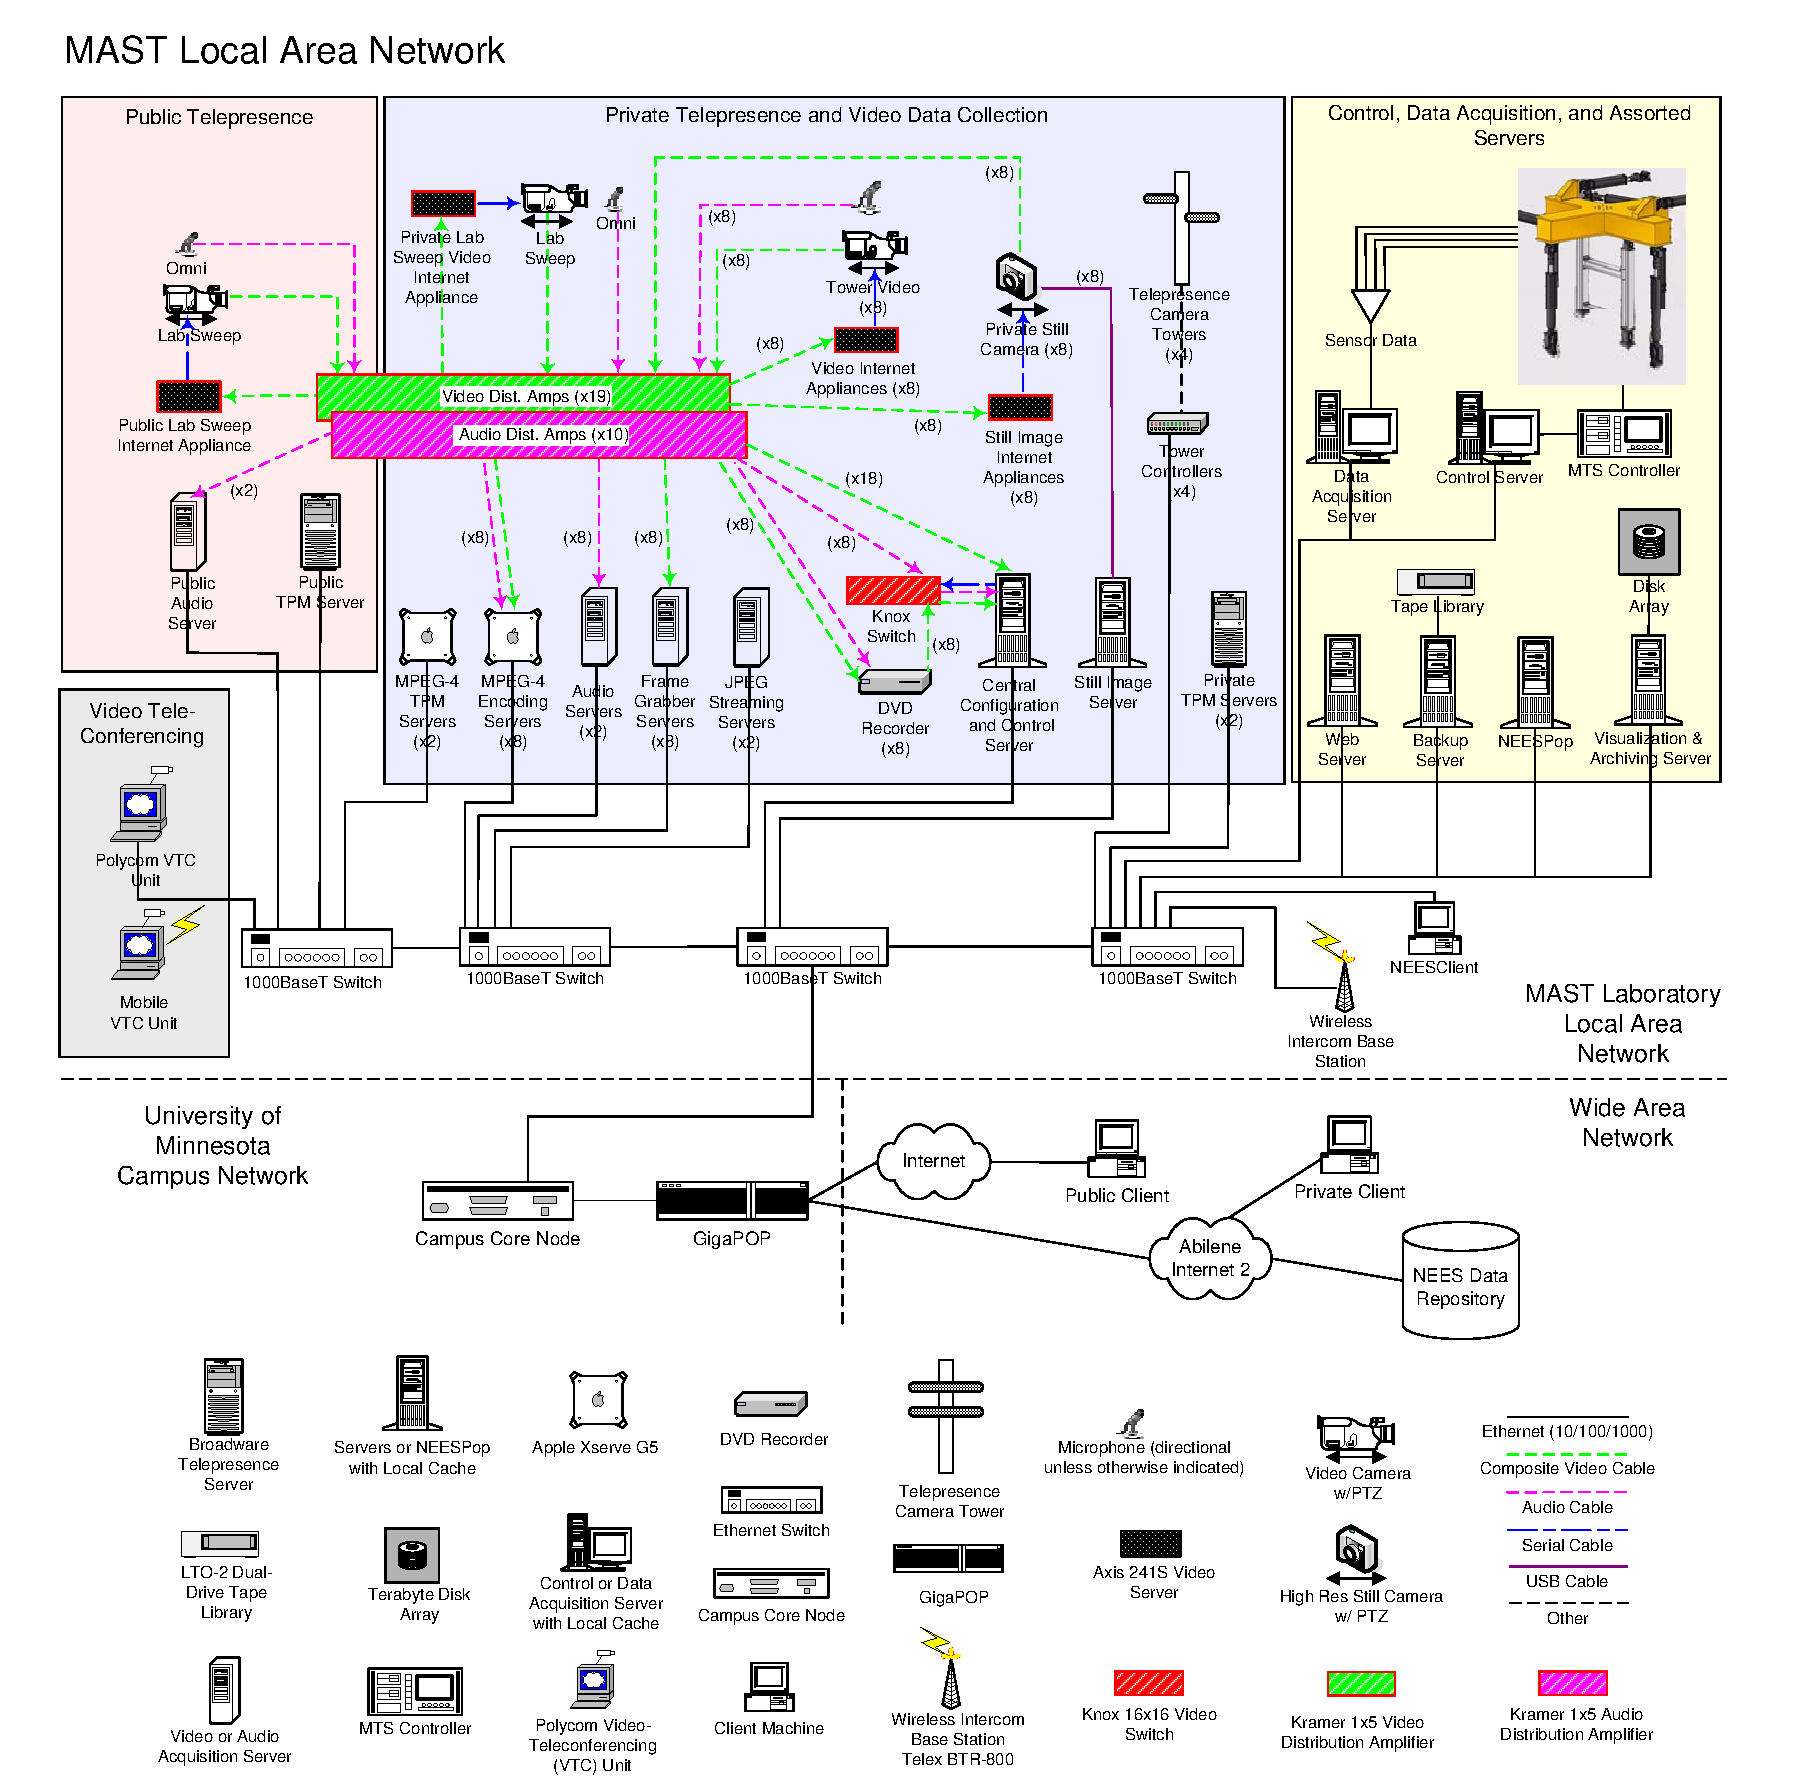
\includegraphics[scale=0.50]{figs/MAST}
% \end{center}
\caption{\label{fig:mast-arch}MAST laboratory network architecture}
\end{figure*}

%(Figure~\ref{fig:ucla-arch})
We deployed RBNB DataTurbine for in a laboratory that conducts Multi-Axial Subassemblage Testing
(MAST) experiments. This is a large-scale test facility, with experiments that may run continuously for a week or more. Experiments are collaborative with remote institutions even spanning multiple countries.
% The MAST (Multi-Axial Subassemblage Testing) lab ~\cite{mast} at the University of Minnesota is a large-scale test facility, with experiments that may run continuously for a week or more. Experiments are collaborative with remote institutions such as the University of Iowa and the University of Puerto Rico at Mayaguez. 
Remote collaboration is thus a requirement and priority. As can be seen in Figure ~\ref{fig:mast-arch}, the local network configuration is extremely complex and highly optimized. 

The MAST lab has 384 channels of data acquisition, running on a National Instruments platform and sampling at 1Hz. This includes data from 256 channel strain gages and 192 channels of voltage inputs (mainly string potentiometers and LVDTs for position measurements). There are eight high-resolution still cameras, one at each corner of the lab floor, mounted on remote-controlled towers. These cameras are used to capture 4 megapixel images of samples as the test progresses, with data annotated by custom code (rewriting the EXIF header) before sending it to the Data Turbine.  Eight of these cameras are on robots, and two permanently mounted with views of the lab floor. There are also ten telepresence (NTSC-resolution) cameras on pan-tilt-zoom (PTZ) platforms to provide remote participants with a sense of the state of the lab and experiment. The camera towers and PTZ cameras also have audio microphones, where the sampled sound is streamed out via the Data Turbine, which accounts for ten channels of audio from the floor. The goal was to deploy RBNB DataTurbine  for data acquisition
from the aforementioned sensors and support streaming with mirroring to remote sites for collaboration. 

\emph{Lessons Learned}

We encountered significant unexpected problems in this experiment. 
\begin{enumerate}
\item NTP was not working properly on all connected systems. This was straightforward to correct.
\item The mirroring to Iowa would fail quickly, with poor performance beforehand. The university campus was using a packet shaper, which decided that RBNB DataTurbine traffic was peer-to-peer file sharing. This meant that RBNB was experiencing more than 70\% packet loss, causing the mirroring to fail. The fix for this required intervention by the % UMN 
campus networking personnel.
\item The % UMN 
Internet2 router was unable to handle the traffic that RBNB generated, and would fail in unpredictable ways. An upgrade was required to solve this.
\item The initial design included multiple machines each hosting an RBNB server; after deployment experience a single quad-CPU (2.8GHz, 4GB RAM) machine running a single RBNB server is used instead. This has sufficient resources and is simpler to administrate and configure. This RBNB server is able to archive about two weeks' worth of data to a 1.2TB RAID array, with all 300+ DAQ channels and video sampled at 1Hz.
\item Java version 1.42 had stability problems, where ten clients would cause problems with server stability. These were resolved in JDK 1.5, and subsequent remote stress testing to another university was problem-free.
\end{enumerate}

The overarching lessons are that data streaming will place unusual demands on the network, and that expertise is required to diagnose and correct the resulting problems. However, once these problems were fixed, we were able to stream data and the system is in production today. 


\subsection{NEON Single-String Diagnostic Testbed}

To validate various aspects of the NEON architecture with working prototypes, 
NEON Single-String Diagnostic Testbed (SSTB) activity was initiated. Please 
refer to the single-string diagnostic testbed document for further details on
deployment experience.

% \subsection{NEON Single String Testbed}
The National Ecological Observatory Network (NEON) is an designed to facilitate an advanced understanding of how ecosystems and organisms respond to variations in climate and changes 
in land use. To validate various aspects of the NEON architecture with working prototypes, 
NEON Single-String Diagnostic Testbed (SSTB) activity was initiated. We now describe SSTB and explain how we have used RBNB DataTurbine in this deployment. The goal of the SSTB activity was to develop an end-to-end prototype that streams data from the NEON Wireless Platform (NWP) deployed at a field station 
% UCR/James Reserve
 using a streaming data middleware to a database system deployed at a data center. Figure~\ref{fig: ssarch} shows where individual components are
located -- in field station and data center. The field station and the data center are about 
100 miles apart from each other.
% San Diego Supercomputer Center. 

\begin{figure*}
% \begin{center}
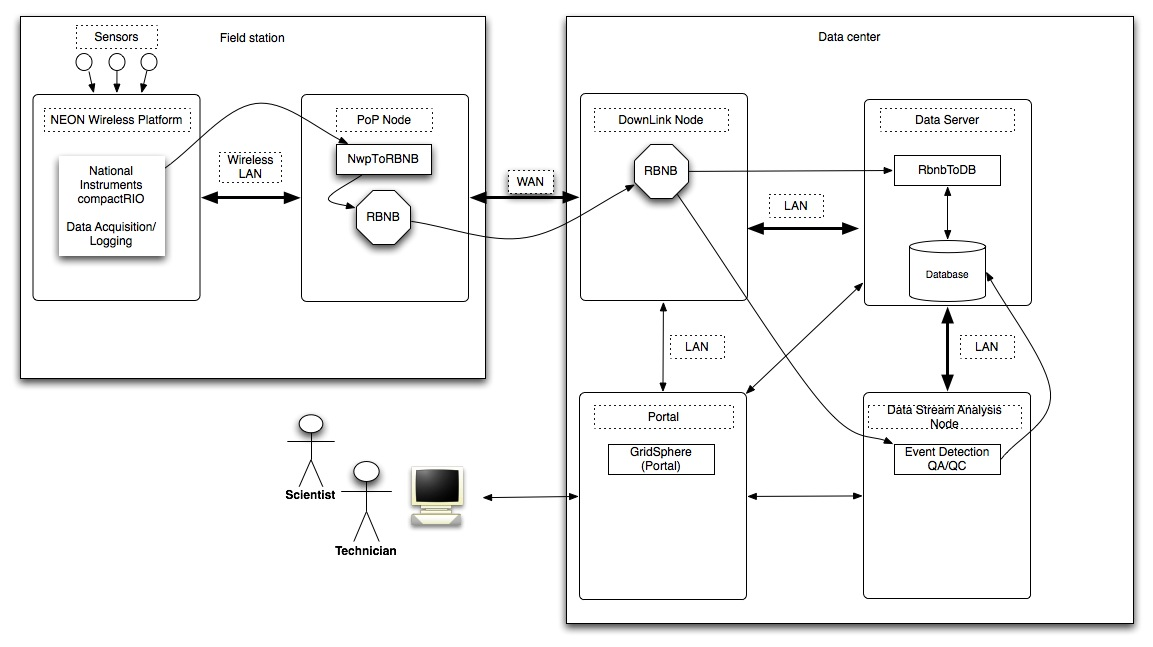
\includegraphics[scale=0.40]{figs/ssarch}
% \end{center}
\caption{\label{fig: ssarch}
NEON Single String Testbed}
\end{figure*}

The Compact RIO is an embedded data acquisition platform manufactured by National Instruments.
In the prototype phase, a Compact RIO datalogger with wireless (802.11b) extensions has been selected as the NEON Wireless Platform (NWP) for  data acquisition system for prototyping. As a part of SST activity, our collaborators deployed a NWP along with Vaisala Weather Transmitter WXT510 and Vaisala Digital Barometric Pressure Sensor (PTB210) at the the field station. Our collaborators 
developed the device driver in LabVIEW for collecting data from the aforementioned sensors connected to the NWP. We deployed PoP node  at the field station. The PoP node hosts an RBNB server and a RBNB source program called NwpToRbnb (ref. Figure~\ref{fig: ssarch}). NwpToRbnb is a Java program that acts as a gateway and facilitates dataflow from the NWP to the RBNB server on the PoP node. It accomplishes this by querying the NWP for data and metadata, processing these items, and then forwarding this data and metadata to the RBNB server deployed on the PoP node. This program initiates the connection with the NWP using sockets and uses standard TCP/IP networking protocols to communicate with the NWP over the wireless channel. Once the session is established, then data is transmitted in an event-driven manner from the NWP to the PoP. 

\emph{Downlink Node:} This 
 % -- San Diego Supercomputer Center. Downlink node
hosts a RBNB server, which runs as the parent node for the RBNB server running on the PoP node. RBNB server running on the downlink node provides access to real-time data streams for various clients. For example, as shown in Figure~\ref{fig: ssarch}, we can fork data streams from the RBNB server running at the downlink node to applications running on the data stream analysis node and data server node.
	
\emph{Data Server node:} This hosts a PostgreSQL database. RbnbToDb is a DataTurbine sink (ref. Figure~\ref{fig: ssarch})that runs in subscription mode. RbnbToDb program connects to RBNB server on the downlink node, extracts the data and then inserts it into the database. RbnbToDb utilizes the JDBC abstraction layer, so the use of Postgres is subject to later revision as requirements change.

\emph{Data stream analysis node:}
 We are currently working on providing this functionality. This node is designed to host software infrastructure that can perform analysis on real-time data streams. An example of such software is Kepler~\cite{kepler} and examples of analysis routines are event detection and QA/QC.
 
\emph{Web Portal node:}
Web portal node hosts the portal software infrastructure. We have deployed a GridSphere-based portal infrastructure, with portlets to support different functions, e.g. for login, and data access/display.

At present the RBNB servers running on the PoP node and the downlink node have been
buffering approximately  one weeks' worth of data. So far in this deployment we have found RBNB DataTurbine to be very robust.



